%----------------------------------------------------------------------------------------
%	PACKAGES AND DOCUMENT CONFIGURATIONS
%----------------------------------------------------------------------------------------
\documentclass[11pt]{article}
\usepackage{amsmath} % Required for some math elements
\usepackage[usenames,dvipsnames]{xcolor}
\usepackage{lipsum} 
\usepackage{cite}
\usepackage{graphicx} % Required for the inclusion of images
\usepackage{algorithmic}
\usepackage{array}
\usepackage{bookmark}
\usepackage{listings}
\usepackage{amssymb}
\usepackage{enumitem}
\usepackage[margin=24mm]{geometry}
\usepackage[caption=false, font=footnotesize]{subfig}
\usepackage{multirow}
\usepackage{hyperref} 


\newlist{steps}{enumerate}{1}
\setlist[steps, 1]{label = Step \arabic*:}

\hypersetup{ %color attributes of citation, link, etc.
    colorlinks=true,
    linkcolor=blue,
    filecolor=gray,      
    urlcolor=blue,
    citecolor=blue,
}

 
\lstdefinelanguage{VHDL}{
    morekeywords=[1]{
        library,use,all,entity,is,port,in,out,end,architecture,of,begin,and,or,Not,downto,ALL
    },
    morekeywords=[2]{
        STD_LOGIC_VECTOR,STD_LOGIC,IEEE,STD_LOGIC_1164,NUMERIC_STD,STD_LOGIC_ARITH,STD_LOGIC_UNSIGNED,std_logic_vector,std_logic
    },
    morecomment=[l]--
}

\definecolor{keyword}{rgb}{0,0.3,0.7}
\definecolor{STD}{rgb}{0.9,0.0,0.7}
\definecolor{comment}{rgb}{0.0,0.6,0.1}

\lstdefinestyle{vhdl}{
   language     = VHDL,
   basicstyle   = \footnotesize\ttfamily,
   keywordstyle = [1]\color{keyword}\bfseries,
   keywordstyle = [2]\color{STD}\bfseries,
   commentstyle = \color{comment}
   breaklines=true,                % sets automatic line breaking
   tabsize=3		                   % sets default tabsize to 2 spaces
}


\newcommand{\matlab}{\textsc{Matlab }} %very important and totally necessary addition

\newcommand\Item[1][]{%
    \ifx\relax#1\relax  \item \else \item[#1] \fi
    \abovedisplayskip=0pt\abovedisplayshortskip=0pt~\vspace*{-\baselineskip}}
%----------------------------------------------------------------------------------------
%	DOCUMENT INFORMATION
%----------------------------------------------------------------------------------------
 
\title{ECEN302 : Embedded Systems \\ Assignment 3 Submission}
\author{Daniel Eisen : 300447549}
\date{\today}

\begin{document}
    \maketitle
    %----------------------------------------------------------------------------------------
    %	DOCUMENT CONTENT
    %----------------------------------------------------------------------------------------
    \begin{enumerate}
        \item \textit{\textbf{You have been asked to design a circuit that can digitize a ±1 V audio signal, band limited to 16 kHz, to within a precision of 50uV. Discuss the key issues here in considering what ADC to use and then suggest a commercially available ADC.}}

              For selection of a suitable ADC, the sample rate must be fast enough to enable the capture of the full bandwidth without aliasing, i.e. rated for at or above 16kMhz. It must have a enough output bits to meet the precision required for the given input range and given that is an audio application should not be too noisy.
              Note that the input signal can be amplified to match the full input range of the selected ADC to preserve precision.

            The AD677 is a 16 bit, 1Mhz, $\pm$5V Sampling ADC.

        \item \textit{\textbf{Briefly describe the type of ADC typically used in a digital voltmeter or weigh scale. Describe how this type of convertor can reject 50 Hz mains interference.}}

              This a Duel Slope ADC. Which operated by first integrating $V_{in}$ for a constant time ($T_{int}$), after which $-V_{ref}$ [note that $|V_{ref}| > |V_{in}|$] is integrated until the output of the integrator reach's zero again. I.e. a variable slope for a set time against a set slope for a variable time (T2). As the second slope and first integration time are constant the input measured voltage is directly proportional to the second integration time. This is relative measure so eliminates affect of changing RC.

              As the average value of a sinusoidal signal is 0V, setting $T_{int}$ such that in integer number of cycles occur in this time eliminates the interference as this is time where an external signal.

        \item \textit{\textbf{Briefly describe the operation of a sample and hold unit and suggest when such a device is required. Choose a suitable S\&H for the application described in question 1 above, given that an ADC without a S\&H was chosen}}

              A Sample and Hold unit takes a snapshot of an instantaneous voltage signal and holds that voltage for as long as is required. This values can then be read in an ADC for example.

              The LF198/398 meets the input range requirement, low output noise and wide bandwidth.

        \item \textit{\textbf{What is the quantisation error of a 12 bit Analogue to Digital converter with an input voltage range of 0 to +1V.}}

              $1V/2^{12}=244.14 \mu V \therefore \mathrm{quantisation \; error} \approx \pm 122 \mu V$

              \newpage
        \item \textit{\textbf{A 16-bit successive approximation ADC with an input voltage range of $\pm$5V is connected to a 16 MHz clock. This ADC is used to convert an input signal of 2.1362V. Determine the digital output and the time for the conversion.}}

              Take 16 'guesses', one per clock cycle, therefore the conversion time is $1\mu S$.

              To get nearest output value, assuming 0b0... is -5V:

              $$\frac{2.136+5}{\frac{10}{2^{16}}} \approx 46768$$

        \item \textit{\textbf{Sketch a block diagram of a Delta-Sigma ADC and then describe:}}

              \begin{center}
                  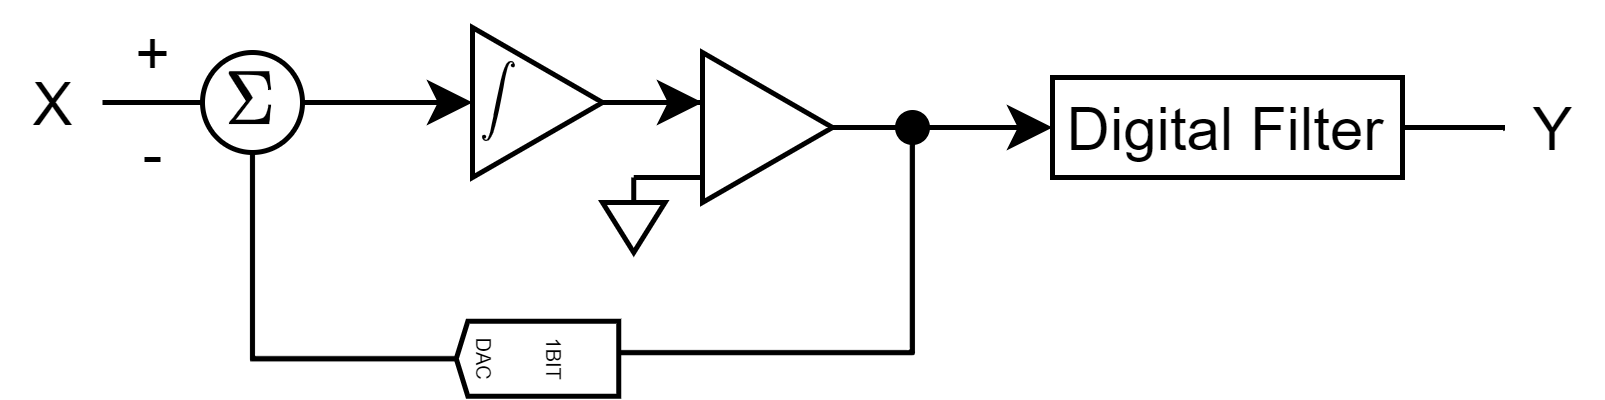
\includegraphics[width=0.75\textwidth]{inc/del-sig.png}
              \end{center}

              \begin{enumerate}
                  \item \textit{The signal that comes out of the comparator and how it relates to the input voltage.}

                        The output of the comparator is a serial PWM signal whose proportion of high to low levels is representative of Vin (compared to the input range).

                  \item \textit{How this comparator output signal is then converted into a multi-bit digital output.}

                        This signal is then digitally filtered, by oversampling it considerably into a bitstream, taking a rolling average of the bitstream to extract a binary digital value.

              \end{enumerate}
    \end{enumerate}

\end{document}